\section{Arduino}
\subsection{Pengertian Arduino}
Arduino merupakan sebuah perangkat mikro dari Singleboard yang bersifat Opensource yang berasal dari platform Wiring yang kemudian dirancang untuk dapat memudahkan para penggunaan elektronik di setiap bidang. Perangkat kerasnya memiliki prosesor AVR Atmel, nama AVR sendiri berasal dari nama prosesor Alf Egil Bogen dan Risc Vegard Wollan di mana Alf Egil Bogen dan Vegard Wollan adalah dua penemu yang berasal dari Norwegia yang menemukan mikrokontroler AVR yang kemudian dipasarkan oleh Atmel, dan perangkat lunaknya tersebut memiliki bahasa pemrograman tersendiri. 
Arduino juga merupakan platform perangkat keras terbuka yang ditujukan untuk siapa pun dan kalangan apapun yang ingin membuat prototip peralatan elektronik interaktif berdasarkan perangkat keras dan perangkat lunak yang fleksibel dan mudah digunakan. Perangkat dari mikrokontroler deprogram atau dibuat menggunakan bahasa pemrograman arduino yang memiliki kesamaan atau kemiripan dengan bahasa pemrograman C, karena bersifat terbuka dapat mendownload skema hardware arduino dan membangunnya. 
Arduino menggunakan keluarga mikrokontroler ATMega yang dilepaskan Atmel sebagai basis, namun ada individu perusahaan yang membuat klon arduino menggunakan mikrokontroler lainnya dan tetap kompatibel dengan arduino di tingkat perangkat keras. Agar bisa, program dimuatkan melalui bootloader meski ada pilihan untuk bypass bootloader dan menggunakan downloader untuk memprogram mikrokontroler secara langsung melalui port ISP.

\begin{figure}[ht]
	\centerline{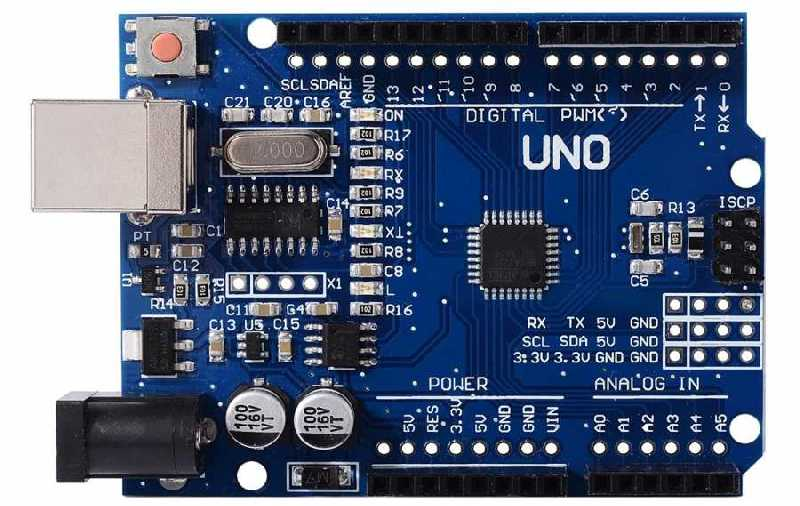
\includegraphics[width=1\textwidth]{figures/arduino.jpg}}
	\caption{Arduino}
	\label{Arduino}
	\end{figure}

\subsection{Sejarah Arduino}
Semuanya dimulai dengan tesis yang dibuat oleh Hernando Barragan, di institut Ivrea, Italia pada tahun 2005, dikembangkan oleh Massimo Banzi dan David Cuartielles dan dinamai Arduin dari Ivrea. Kemudian berganti nama menjadi Arduino yang di Italia berarti teman yang pemberani.
Tujuan awal Arduino adalah membuat perangkat mudah dan murah, dari perangkat yang ada saat itu. Dan perangkat ini diperuntukkan bagi siswa yang akan membuat perangkat desain dan interaksi.
Empat hal dalam bahasa Arduino ini:
\begin{enumerate}
\item Harga terjangkau
\item Bisa dijalankan di berbagai sistem operasi, Windows, Linux, Max, dan sebagainya.
\item Sederhana, dengan bahasa pemrograman yang mudah dipelajari oleh orang awam, bukan untuk orang teknis saja.
\item Open Source, perangkat keras dan perangkat lunak.
\end{enumerate}
Sifat Arduino dari Open Source, membuat Arduino tumbuh sangat cepat. Dan banyak perangkat kelahiran seperti Arduino. Contohnya seperti DFRDuino atau Freeduino yang terus memiliki MurmerDuino yang diciptakan oleh Robot Unyil, ada AViShaDuino lainnya yang salah satu penciptanya yaitu Admin Kelas Robot.
Sampai sekarang ini resmi telah membuat berbagai jenis Arduino yang baru. Mulai dari yang paling mudah didapatkan sehingga banyak digunakan oleh para user, contohnya yaitu Arduino Uno. Arduino yang sudah menggunakan ARM Cortex berbentuk Mini PC. Pada arduino menggunakan bahasa pemrograman C yang telah disederhanakan. Sehingga setiap orang yang baru belajar menggunakan arduino bisa menggunakannya dan bisa menjadi seniman digital.

\subsection{jenis-jenis Arduino}
Arduino Uno R3
Arduino Uno R3 adalah boardsistem minimum berbasis mikrokontroller ATmega328P jenis AVR. Arduino Uno R3 memiliki 14 digital input output 6 diantaranya dapat digunakan untuk PWM output, 6 analog input, 16 MHz osilator kristal, USB connection, power jack, ICSP header dan tombol reset. Skema dari Arduino Uno R3 dengan
karekteristik sebagai berikut:
\begin{itemize}
\item Operating voltage 5 VDC.

\item Rekomendasi input voltage 7-12
VDC
\item Batas input voltage 6-20 VDC.
\item Memiliki 14 buah input output digital.
\item Memiliki 6 buah input analog.
\item DC Current setiap I O Pin sebesar 40mA.
\item DC Current untuk 3.3V Pin sebesar 50mA.
\item Flash memory 32 KB.
\item SRAM sebesar 2 KB.
\item EEPROM sebesar 1 KB.
\item 11 Clock Speed 16 MHz.
\end{itemize}

\subsection{Kerja Arduino}
Dengan beberapa dasar-dasar listrik, Arduino, dan robot.
contoh kode menggunakan komponen berdaya rendah dapat dihubungkan langsung ke Arduino LED, potensiometer, penerima R C, tombol switch, dan sebagainya. 
Bab ini berfokus pada bagaimana menghubungkan Arduino dengan switch mekanis, elektronik, dan optik, serta beberapa metode kontrol masukan yang berbeda, dan akhirnya beberapa pembicaraan tentang sensor.

\subsection{Anatomi Jaringan Sensor}
Jaringan sensor ada dimana-mana. Mereka biasanya dianggap sebagai sistem pemantauan manufaktur yang rumit
dan aplikasi medis. Namun, mereka tidak selalu rumit, dan mereka ada di sekitar Anda.
Di bagian ini. kita akan memeriksa blok bangunan dari jaringan sensor. dan bagaimana mereka terhubung secara logis.
pertama mari kita lihat contoh dari jaringan sensor dalam upaya memvisualisasikan komponennya.

\subsection{Mengapa menggunakan Arduino?}
Fleksibel, menawarkan beragam input digital dan analog, SPI dan interface serial serta digital dan PWM
output. Mudah digunakan, terhubung ke komputer via USB dan berkomunikasi menggunakan protokol serial standar, berjalan
dalam mode standalone dan sebagai antarmuka yang terhubung ke komputer PC  Macintosh
Ini tidak mahal, sekitar 30 dollar per papan dan dilengkapi dengan perangkat lunak authoring gratis. Ini adalah proyek sumber terbuka,
Perangkat lunak  perangkat keras sangat mudah diakses dan sangat fleksibel untuk disesuaikan dan diperluas. Arduino didukung
oleh komunitas online yang berkembang, banyak sumber sudah tersedia.

\subsection{Arduino berinteraksi dengan Softwares}
Arduino dapat berbicara, mentransmisikan atau menerima data melalui saluran serial, jadi perangkat lain dengan serial
Kemampuan bisa berkomunikasi dengan Arduino. Tidak masalah bahasa program pemrograman apa yang sedang mengemudi
perangkat lainnya Anda bisa menggunakan port serial utama Arduino, yang digunakan saat Anda berbicara dengannya
program itu, atau Anda dapat meninggalkan saluran yang didedikasikan untuk pemrograman dan serial lingkungan pengembangan
monitor, dan gunakan dua pin lainnya untuk link serial tambahan yang didedikasikan untuk perangkat eksternal. Beberapa program seperti
Flash tidak memiliki kemampuan serial asli. Mereka masih bisa berkomunikasi dengan Arduino melalui perantara
yang, seperti penerjemah, memungkinkan mereka berbicara satu sama lain.

\subsection{Algoritma berbasis arduino} 
yang terinspirasi oleh perilaku pencarian hewan diajukan, dianalisis dan diimplementasikan. Algoritma lokalisasi didistribusikan; range based dan menggunakan Xbee arduino mengatur untuk menghitung jarak antara node jangkar dan node sensor. Karena algoritma terdistribusi maka komunikasi informasi lokasi ke sink node melalui beberapa SN berkurang. Hal ini membuat algoritma hemat energi sehingga lifetime, reliability dan kinerja jaringan sensor nirkabel semakin meningkat. Algoritma ini mudah diterapkan, memiliki ketepatan keluaran yang masuk akal, dan konvergensi yang lebih baik. Algoritma ini dapat lebih ditingkatkan dengan menyetel parameter desain, dengan mengurangi kesalahan RSSI dengan desain dan penempatan yang tepat dari setup arduino Xbee. Algoritma hybrid lebih lanjut dapat dipelajari dan dianalisis untuk meningkatkan akurasi dan konvergensi.

\subsubsection{Arduino Mega}
Arduino Mega adalah papan mikrokontroler berdasarkan ATmega1280 datasheet. Ini memiliki 54 pin input atau output digital, 16 input analog, 4 UART port serial perangkat keras, osilator kristal 16 MHz, koneksi USB, colokan listrik, header ICSP, dan tombol reset. Ini berisi semua yang dibutuhkan untuk mendukung mikrokontroler; cukup hubungkan ke komputer dengan kabel USB atau nyalakan dengan adaptor AC-ke-DC atau baterai untuk memulai. Mega kompatibel dengan kebanyakan perisai yang dirancang untuk Arduino Duemilanove atau Diecimila.

\subsection{sistem arsitektur}
Desain yang diusulkan untuk sistem Pelaporan Kualitas Air Ubiquitous mobile u-WQR untuk penginderaan di tempat
dan melaporkan data kualitas air disajikan. Sistem ini dikembangkan sebagai salah satu komponen tata kelola air
sistem dirancang untuk menangani tantangan pengelolaan air di sekitar Danau Victoria Basin.
Meskipun teknik dan teknologi yang lebih maju sudah ada di dunia, sistem u-WQR diterapkan
menggunakan teknologi yang lebih sederhana dan open source untuk mengurangi biaya sistem.

\subsubsection{Power}
Arduino Mega dapat bertenaga melalui koneksi USB atau dengan catu daya eksternal. Sumber daya dipilih secara otomatis.

Daya eksternal non-USB bisa datang baik dari adaptor AC-ke-DC kutil dinding atau baterai. Adaptor dapat dihubungkan dengan memasang steker positif pusat 2.1mm ke soket daya board.

Pin Power adalah sebagai berikut:
\begin{itemize}
\item VIN. Tegangan masukan ke papan Arduino saat menggunakan sumber daya eksternal berlawanan dengan 5 volt dari koneksi USB atau sumber daya yang diatur lainnya. Anda bisa mensuplai voltase melalui pin ini, atau jika mensuplai voltase melalui colokan listrik, akseslah melalui pin ini.
\item 5V. Catu daya yang diatur digunakan untuk menyalakan mikrokontroler dan komponen lainnya di papan tulis. Ini bisa datang baik dari VIN melalui regulator onboard, atau disediakan oleh USB atau suplai 5V yang diatur lainnya.
\item 3V3 Pasokan 3,3 volt dihasilkan oleh chip FTDI onboard.
\item GND. Ground pin
\end{itemize}


\subsubsection{communication}

Sebuah perangkat lunak Serial library memungkinkan komunikasi serial pada salah satu pin digital Mega.

ATmega1280 juga mendukung komunikasi I2C dan SPI.

\subsubsection{Karakteristik Fisik dan Kompatibilitas}

Perhatikan bahwa jarak antara pin 7 dan 8 digital adalah 160 mil, bukan kelipatan jarak 100 mil dari pin lainnya.

Mega dirancang agar kompatibel dengan sebagian besar perisai yang dirancang untuk Diecimila atau Duemilanove. Pin digital 0 sampai 13 pin AREF dan GND yang berdekatan, input analog 0 sampai 5, soket daya, dan header ICSP semuanya berada pada lokasi yang setara. SPI tersedia melalui header ICSP pada Mega dan Duemilanove  Diecimila. Harap dicatat bahwa I2C tidak terletak pada pin yang sama pada Mega 20 dan 21 sebagai Duemilanove  Diecimila input analog 4 dan 5.

\subsubsection{Perlindungan Overcurrent USB}

Arduino Mega memiliki polibak yang dapat disetel ulang yang melindungi port USB komputer Anda dari celana pendek dan arus lebih.Jika lebih dari 500 mA diterapkan ke port USB, sekering akan secara otomatis memutus koneksi sampai pendek atau overload dilepaskan.
\subsection{Sensor}
Sensor adalah perangkat elektronik yang mengukur kualitas fisik seperti cahaya atau
suhu dan mengubahnya menjadi tegangan. Proses ini mengubah satu bentuk energi
ke yang lain disebut transduksi. Seringkali, sensor juga disebut sebagai transduser.
Sensor dapat diklasifikasikan secara luas dalam dua kategori: sensor digital dan sensor analog.
Output sensor digital hanya bisa berada di salah satu dari dua keadaan yang mungkin terjadi. Ini adalah ON
sering + 5V, atau OFF, 0V. Sebagian besar sensor digital bekerja dengan ambang batas. Apakah yang masuk
Pengukuran di bawah ambang batas, sensor akan mengeluarkan satu keadaan, apakah berada di atas
Ambang batas, sensor akan menampilkan keadaan yang lain.

\subsection{Sensor DHT 11}
Sensor ini merupakan sensor dengan kalibrasi sinyal digital yang mampu memberikan informasi suhu dan kelembaban. Sensor ini tergolong komponen yang memiliki tingkat stabilitas yang sangat baik. Sensor ini termasuk elemen resistif dan perangkat pengukur suhu NTC.

\subsection{Perekam Data (Data Logger)}
Perekam Data disebut juga data logger. Secara umum perekam data sederhana terdiri dari mikrokontroller,sensor dan media penyimpanan. Kemudian Data ini nantinya akan
tersimpan didalam media penyimpanan yaitu memory card. Pada perancangan ini jenis memory card yang akan digunakan adalah micro SD 
Secure Digital dengan kapasitas 4 GB.

\subsection{Topologi Jaringan}
Sistem pemantauan dan pengukuran jarak jauh terdiri dari 2 buah modul 
Xbee Proyang sama yang sebelumnya telah diprogram sebagai sebuah receiver-transmiter maupun transmiter-receiver. Ada beberapa bentuk topologi yang biasa digunakan antara lain topologi mesh, peer, star, dan cluster Tree.
Topologi pair merupakan jaringan yang sederhana dengan hanya menggunakan dua buah xbeeatau node. Satu node harus menjadi coordinator sehingga jaringan dapat dibentuk. Dan yang lain dikonfigurasikan sebagai routeratau perangkat akhir.

Cara yang saat ini banyak digunakan  dalam topologi jaringan adalah bus, token ring, dan star yaitu:
\begin{itemize}
\item Topologi BUS 
Topologi bus terlihat pada Gambar 2. Media penghantar untuk jenis topologi BUS adalah kabel Koaksial. Topologi BUS menggunakan metode unicast, multicastdan broadcast. Unicastadalah komu- nikasi antara satu pengirim 
dengan satu penerima di jaringan. Multicastadalah komunikasi antara satu pengirim dengan banyak penerima di jaringan. Sedangkan pada Broadcast, setiap titik akan menerima dan menyimpan frameyang disalurkan/dihantarkan.

\item Topologi Token RING 
Topologi Token RING adalah. Metode token-ring sering disebut ringsaja menghu-bungkan komputer sehingga ber-bentuk ring (lingkaran). Setiap 

\item Topologi STAR 
Topologi ini merupakan kontrol terpusat, semua link harus melewati pusat yang menyalurkan data tersebut kesemua simpul atau clientyang dipilihnya. Simpul pusat dinamakan stasiun primer atau 
server dan lainnya dinamakan 

\end{itemize}
\subsubsection {Arduino 1.0.1 dan XCTU}

Arduino merupakan perangkatpemrograman mikrokontroller jenis Atmel yang tersedia secara bebas open-source
dengan menggunakan bahasapemrograman C. Untuk menyelesaikan rangkaian agar bisa bekerja, maka langkah selanjutnya adalah membuat program yang
akan diupload ke board Arduino.Penelitian ini menggunakan software Arduino 1.0.1untuk membuat program pada sketch Arduino kemudian diverify
untuk memastikan program sudah benar,selanjutnya program di upload. Setelah program di upload dan tidak ada kesalahan
maka akan tampil done uploading. Untuk mengaplikasikan program pada sistem telemetri ini maka dibutuhkan perangkat lunak yang untuk men-setting atau pun pemberian alamat pada Xbee Pro untuk melakukan komunikasi antara unit pengirim dan unit penerima. Adapun
perangkat lunak yang di gunakan adalah perangkat lunak X-CTU, yaitu perangkat lunak dari produk Xbee Pro

\subsection  {I/O Expansion Shield Arduino}
I/O Expansion Shield untuk Arduino adalah perangkat tambahan yang digunakan untuk interface beberapa modul yang compatible dengan board arduino. Board I/O expansion ini memiliki inputtegangan 5 VDC. Modul- modul yang cocok dan sesuai dengan board Arduino dapat mendukung RS485. Xbee Pro, APC220, SD Card dan Bloetooth.

\subsection {Xbee Pro}
Xbee Pro merupakan modul yang memungkinkan Arduino Uno untuk berkomunikasi secara wireless
mengunakan protocol ZigBee. ZigBee beroperasi menggunakan pada spesifikasi IEEE 802.15.4 beroperasi pada frekuensi
2.4 GHz, 900 dan 868 MHz. XBee Pro dapat digunakan sebagai pengganti kabel serial.Xbee Pro diharapkan dapat memperkecil biaya dan menjadi
konektivitas berdaya rendah untuk peralatan yang memerlukan baterai untuk hidup selama beberapa bulan sampai beberapa tahun, tetapi tidak memerlukan kecepatan transfer data tinggi. Xbee Pro memungkinkan komunikasi wireless dalam jangkauan hingga 100 meter indoor dan 1500 meter outdoor.

\subsection {JENIS JENIS ARDUINO USB}
Menggunakan USB sebagai antar muka pemrograman atau komunikasi komputer. Contoh:
\begin{itemize} 
\item Arduino Uno
\item Arduino Duemilanove
\item Arduino Diecimila
\item Arduino NG Rev. C
\item Arduino NG Nuova Generazione
\item Arduino Extreme dan Arduino Extreme v2
\item Arduino USB dan Arduino USB v2.0 
\end{itemize}

\subsubsection {ARDUINO NANO DAN ARDUINO MINI}
Papan berbentuk kompak dan digunakan bersama breadboard. Contohnya adalah Arduino Nano 3.0, Arduino Nano 2.x dan Arduino Mini 04, Arduino Mini 03, Arduino Stamp 02


\subsection {ARDUINO SERIAL}
Menggunakan RS232 sebagai antar muka pemrograman atau komunikasi komputer. contohnya adalah Arduino Serial dan Arduino Serial v2.0  

\subsection {ARDUINO MEGA}
Papan Arduino mirip dengan arduino uno dengan spesifikasi yang lebih tinggi, dilengkapi tambahan pin digital, pin analog, port serial dan sebagainya.  Contohnya Arduino Mega dan Arduino Mega 2560  

\subsection {ARDUINO FIO}
Ditujukan untuk penggunaan nirkabel. 

\subsection {ARDUINO LILYPAD}
Papan dengan bentuk yang melingkar. Contoh: 
\begin{itemize}
\item  LilyPad Arduino 00, LilyPad Arduino 01, 
\item LilyPad Arduino 02, LilyPad Arduino 03,
\item LilyPad Arduino 04
\end{itemize}
\subsection {Arduino Leonardo}
Arduino Leonardo adalah papan Mikrokontroler dan didasarkan pada lembar data ATmega32u4. 
Papan Arduino ini memiliki 20 pin input output digital dan dari jumlah pin, tujuh pin digunakan untuk output modulasi lebar pulsa dan 12 pin digunakan sebagai input analog dan ada osilator kristal 16MHz, koneksi USB mikro, RESET pin dan colokan listrik.

Arduino Leonardo ini berisi semua yang dibutuhkan untuk mendukung mikrokontroler; cukup hubungkan ke komputer dengan kabel USB atau nyalakan dengan adaptor AC-ke-DC atau baterai untuk memulai. 
Leonardo berbeda dari semua papan sebelumnya karena ATmega32u4 memiliki komunikasi USB built-in, sehingga menghilangkan kebutuhan akan prosesor sekunder.

Hal ini memungkinkan Arduino Leonardo untuk tampil ke komputer yang terhubung sebagai mouse dan keyboard, selain port COM serial virtual CDC.

\subsection{Arduino Red Board}
Arduino Red Board di program menggunakan kabel USB dari mini-B dengan bantuan dari Arduino IDE Software.

\subsection{Arduino Intel galileo}
Galileo adalah papan mikrokontroler berdasarkanIntel Quark SoC X1000 Application Processor,32-bit sistem Pentium-kelas Intel pada sebuah chip datasheet. Digital pin0-13 dan AREF berdekatan dan pin GND, Analoginput 0 sampai 5, header listrik, ICSP header, danpin port UART 0 dan 1, semua di lokasi yang sama seperti pada Arduino Uno R3. 

Galileo dirancang untuk mendukung shield yang beroperasi di kedua tegangan  3.3V atau 5V.Tegangan operasi inti Galileo adalah 3.3V. Namun,jumper di board memungkinkan terjemahantegangan 5V di pin I  O. Hal ini memberikandukungan untuk 5V shield Uno dan perilaku default.

Tentu saja, board  Galileo juga perangkat lunak yang cocok dengan Arduino Software Development Environment, yang membuatkegunaan dan pengenalan snap. Selain hardwareArduino dan kompatibilitas software, arduino

\subsection{Arduino Pro Micro AT} 
Arduino Mikro Ini memiliki 20 digital pin input output yang 7 dapat digunakan sebagai output PWM dan 12 input analog sebagai, osilator 16 MHz kristal, koneksi USB mikro, header ICSP, dan tombol reset. Dengan  memiliki faktor bentuk yang memungkinkannya untuk dapat dengan mudah ditempatkan pada papan tempat memotong roti.